\documentclass[preprint,12pt,authoryear]{elsarticle}
\usepackage[T1]{fontenc}
\usepackage{lmodern}
\setlength{\emergencystretch}{1em}
\usepackage{amsmath,amssymb,booktabs,graphicx,array,microtype}
\usepackage{xcolor,hyperref}
\usepackage{tikz}
\usetikzlibrary{arrows.meta,positioning,fit,backgrounds}
\hypersetup{colorlinks=true,linkcolor=blue!50!black,citecolor=blue!50!black,urlcolor=blue!50!black}
\newcommand{\todo}[1]{\textcolor{red!70!black}{[TO COMPLETE: #1]}}
\newcommand{\nojepa}{\textsc{NoJEPA}}
\newcommand{\direct}{\textsc{DirectReadout}}
\newcommand{\fullmodel}{\textsc{ForecastAttention}}
\newcommand{\meanmodel}{\textsc{ForecastMean}}
\journal{Medical Image Analysis}
\begin{document}
\begin{frontmatter}
\title{Forecast-aware latent modeling for longitudinal prediction of pathological complete response from breast MRI}
\author{Author information to be completed}
\address{Affiliations and corresponding author to be completed}
\begin{abstract}
Longitudinal breast magnetic resonance imaging (MRI) offers repeated measurements of treatment response, but discriminative models do not necessarily exploit the future disease trajectories implied by an observed examination. We investigate whether auxiliary future-state prediction and an explicit forecast-based readout improve prediction of pathological complete response (pCR). The framework combines three-phase dynamic contrast-enhanced MRI, baseline clinical variables, and assigned treatment-arm scenarios in a latent representation. An autoregressive predictor estimates unobserved future states, and an attention readout summarizes the predicted terminal state and its change from the current state. We study 976 patients with 3,641 usable MRI examinations, using 801 patients for five-fold development and a fixed internal holdout of 175 patients, including 56 pCR-positive cases. Three matched variants isolate direct prediction without future-state supervision, direct prediction with that supervision, and the complete forecast-attention model. This initial analysis reports training seed44, selected retrospectively, and averages metrics from separately evaluated fold models. At T0, T1, and T2, the complete model achieved AUROCs of 0.7294, 0.7381, and 0.7421, respectively. Its three-landmark mean AUROC and average precision were 0.7365 and 0.5990, compared with 0.7219 and 0.5792 for the control without future-state supervision. Direct readout retained the highest mean F1, and forecast attention had worse calibration. Paired patient-bootstrap intervals included zero for the principal model differences. These exploratory findings support further evaluation of forecast-aware representations while motivating independent validation, prospective model selection, and explicit calibration assessment.
\end{abstract}
\begin{keyword}
Breast MRI \sep Pathological complete response \sep Longitudinal imaging \sep Latent dynamics \sep Treatment response prediction
\end{keyword}
\end{frontmatter}
\section{Introduction}
\label{sec:intro}
Neoadjuvant systemic therapy provides an opportunity to monitor breast cancer before surgery and to study how an individual tumor responds over time. Pathological complete response (pCR) is a clinically meaningful endpoint associated with long-term outcomes, although its relationship to prognosis varies across biological subtypes and it should not be equated with a universally valid trial-level surrogate \citep{ctneobc2014}. Predicting pCR from imaging could support response assessment and the design of future adaptive studies. Such a prediction remains a prognostic estimate under an observed treatment context; it does not establish that changing treatment would improve an individual patient's outcome.

Dynamic contrast-enhanced MRI captures three-dimensional anatomy and contrast uptake patterns that evolve during therapy. Prior work in the I-SPY setting has demonstrated associations between MRI-derived tumor measurements and pathological response or subsequent outcomes \citep{hylton2012mri,hylton2016ftv}. Public multicenter imaging resources also make it possible to examine learned representations across repeated visits \citep{tciaispy2_2022,tciaacrin6698_2021}. However, a longitudinal prediction system must operate at the time a decision is considered: a baseline prediction can use baseline information, whereas an interim prediction can use the examination history accumulated by that interim visit. Future scans may inform representation learning on development patients but cannot become inputs to predictions for holdout patients at an earlier landmark.

Most direct classifiers optimize the endpoint of interest from observed images and clinical variables. This is a reasonable objective, but it does not explicitly require the representation to capture how the tumor state may evolve. A different strategy is to predict future imaging information and use the prediction to inform the endpoint readout. Image synthesis provides one route to such a representation, but prediction in a compact latent space can focus the training signal on state evolution without requiring a pixel-space image generator at inference. This distinction is useful for response prediction: the relevant question is whether the learned forecast contributes information to classification, rather than whether a generated image is visually convincing.

Joint-embedding predictive learning offers a general mechanism for predicting target representations computed by a slowly updated encoder \citep{jepa2023}. In a longitudinal medical setting, adapting that principle requires explicit handling of partial histories, missing future observations, treatment context, and the distinction between an auxiliary training target and a classifier input. A model may benefit from a future-state loss while still making a direct prediction from the observed history. Conversely, directly including forecast features in the classifier changes both its information pathway and its parameterization. These effects should be examined through matched controls rather than attributed to a single generic ``world model'' component.

We investigate forecast-aware latent modeling for longitudinal pCR prediction from breast MRI. The model encodes three selected DCE phases at each available visit, fuses observed MRI with baseline clinical information and an assigned treatment-arm scenario, and autonomously rolls the current latent state forward to a terminal stage. A spatial attention mechanism summarizes the predicted terminal state and the predicted change from the current state for pCR classification. We compare the complete model with two direct-readout controls: one without future-state supervision and one with the same auxiliary supervision as the complete model. A supplementary mean-pooling model further examines the attention component.

The study makes three concrete contributions. First, it formulates a common representation and masked future-state objective that can be applied to available T0--T2 histories while using observed later scans only as development-time targets. Second, it provides a staged comparison that distinguishes the effect of auxiliary prediction from the joint effect of forecast readout and attention. Third, it reports landmark-specific discrimination, thresholded classification, calibration, and paired patient-level uncertainty on a fixed internal holdout. The initial manuscript follows a single, retrospectively selected training seed, seed44. Accordingly, the results are presented as an exploratory internal evaluation, with the limits of seed selection and upstream data independence stated explicitly.

\section{Related work}
\label{sec:related}
\paragraph{MRI biomarkers and learned pCR prediction.}
MRI-based response assessment has a substantial clinical and quantitative foundation. Functional tumor volume and related measurements have been studied in longitudinal breast MRI cohorts, including I-SPY \citep{hylton2012mri,hylton2016ftv}. The ACRIN 6698 study additionally examined diffusion-derived measurements in relation to response \citep{ACRIN6698diffusion2018}. These studies motivate imaging-based monitoring but do not establish that a learned model using different inputs or a different evaluation split has equivalent clinical validity. Our experiments use selected DCE phases and baseline clinical variables; diffusion imaging is not an input to the present model.

Learning-based approaches can combine complementary image sequences or repeated examinations. Synthesis-based representation learning has been explored for multi-sequence 3D/4D MRI \citep{han2024synthesis}, and recent studies have examined spatiotemporal or early-treatment information for pCR prediction \citep{tang2025spatiotemporal,du2025early}. Such studies provide relevant methodological context, but differences in patient selection, imaging availability, endpoints, and holdout construction prevent direct numerical comparisons with our results. We therefore do not claim superiority to published systems from cross-paper metric comparisons. Reimplementation of suitable external baselines under the same patient split remains necessary.

\paragraph{Predictive latent representations.}
Predicting a target embedding rather than reconstructing the input image is a central idea in joint-embedding predictive learning \citep{jepa2023}. We use an exponential-moving-average target encoder to define latent states and supervise autonomous future predictions. The present objective is a supervised pCR loss combined with a masked multi-step latent-state loss. It does not activate a separate single-step teacher-forcing JEPA loss, image reconstruction loss, or latent-variance regularizer. This objective-level distinction matters when interpreting the internal experiment name \nojepa{}: that control removes future-state supervision, while retaining the common fusion architecture.

\paragraph{Attention and volumetric image representation.}
Transformer attention provides a flexible way to combine image tokens and contextual information \citep{vaswani2017}. Compact convolutional representations can reduce the cost of processing volumetric MRI, and vector-quantized generative models provide one source of pretrained convolutional encoders \citep{vqgan2021}. Here the pretrained codec contributes a continuous convolutional encoder. The quantizer and image decoder are bypassed, and the main experiments do not synthesize MRI volumes. The final attention weights summarize latent tokens that have already undergone spatial mixing; they are therefore not validated lesion segmentations or anatomical explanations.

\section{Method}
\label{sec:method}
\begin{figure}[t]
\centering
\resizebox{\textwidth}{!}{%
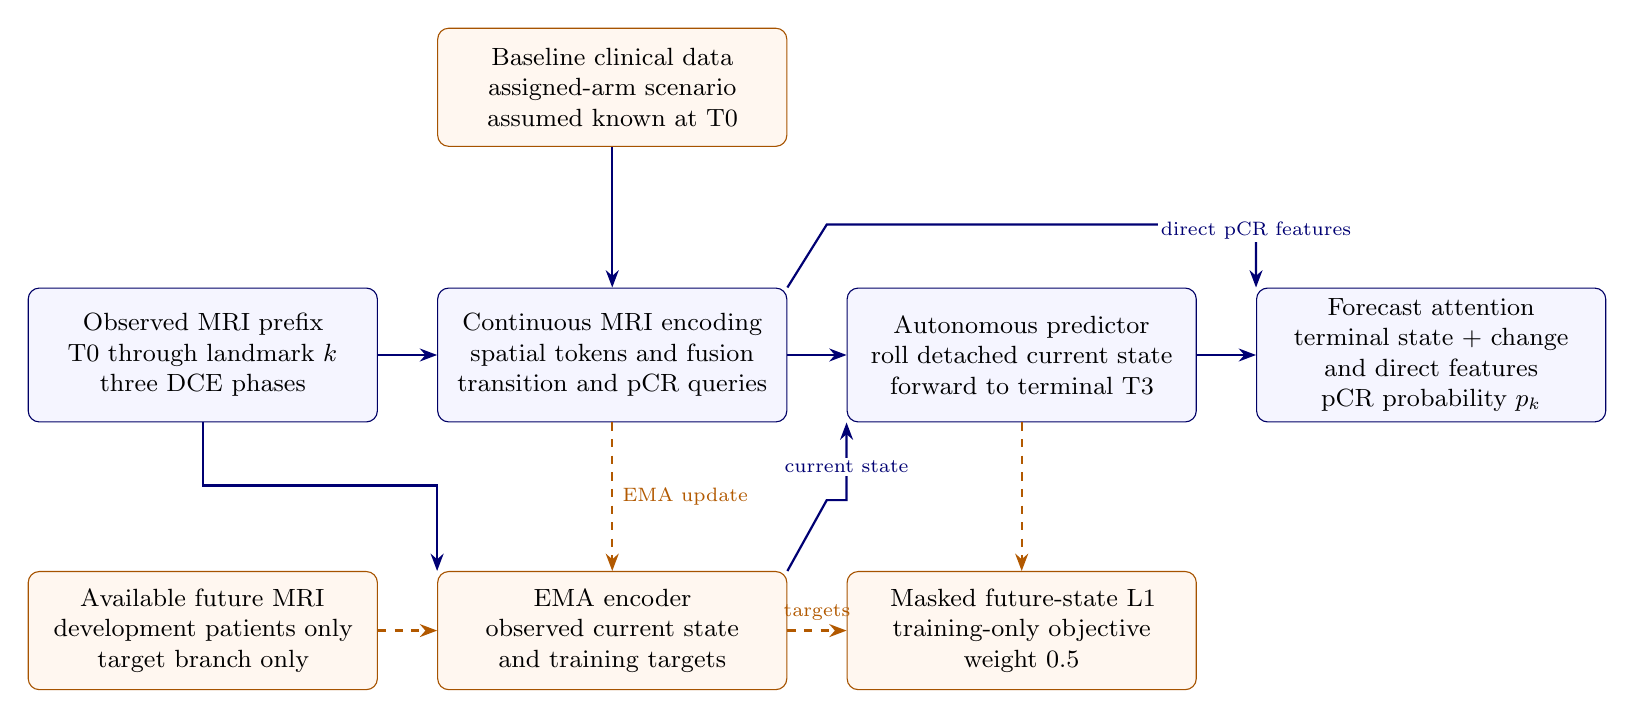
\begin{tikzpicture}[
  box/.style={draw=blue!40!black,rounded corners,fill=blue!4,align=center,minimum height=1.7cm,text width=4.2cm,font=\small},
  aux/.style={draw=orange!65!black,rounded corners,fill=orange!6,align=center,minimum height=1.5cm,text width=4.2cm,font=\small},
  link/.style={-{Stealth[length=2.2mm]},thick,blue!45!black},
  target/.style={-{Stealth[length=2.2mm]},thick,dashed,orange!70!black}]
\node[box] (input) at (0,0) {Observed MRI prefix\\T0 through landmark $k$\\three DCE phases};
\node[box] (encoder) at (5.2,0) {Continuous MRI encoding\\spatial tokens and fusion\\transition and pCR queries};
\node[box] (predictor) at (10.4,0) {Autonomous predictor\\roll detached current state\\forward to terminal T3};
\node[box] (readout) at (15.6,0) {Forecast attention\\terminal state + change\\and direct features\\pCR probability $p_k$};
\draw[link] (input)--(encoder);\draw[link] (encoder)--(predictor);\draw[link] (predictor)--(readout);
\node[aux] (context) at (5.2,3.4) {Baseline clinical data\\assigned-arm scenario\\assumed known at T0};
\draw[link] (context)--(encoder);
\node[aux] (ema) at (5.2,-3.5) {EMA encoder\\observed current state\\and training targets};
\node[aux] (future) at (0,-3.5) {Available future MRI\\development patients only\\target branch only};
\node[aux] (loss) at (10.4,-3.5) {Masked future-state L1\\training-only objective\\weight 0.5};
\draw[target] (encoder)--node[right,font=\scriptsize] {EMA update} (ema);
\draw[target] (future)--(ema);
\draw[link] (input.south) -- ++(0,-.8) -| (ema.north west);
\draw[link] (ema.north east) -- ++(.5,.9) -| node[pos=.65,above,font=\scriptsize,fill=white,inner sep=1pt] {current state} (predictor.south west);
\draw[target] (ema)--node[above,font=\scriptsize] {targets} (loss);
\draw[target] (predictor)--(loss);
\draw[link] (encoder.north east) -- ++(.5,.8) -| node[pos=.65,above,font=\scriptsize,fill=white,inner sep=1pt] {direct pCR features} (readout.north west);
\end{tikzpicture}}
\caption{Conceptual overview of \fullmodel{}. The prediction path uses observed information and an autonomously generated trajectory. The EMA encoder supplies the detached current state; future MRI enters only the training-target branch. The classifier combines direct pCR features with the attention-pooled terminal state and its change from the current state. The diagram summarizes information flow rather than every query or attention-mask connection.}
\label{fig:framework}
\end{figure}


\subsection{Longitudinal prediction problem}
\label{sec:problem}
We consider prediction of pathological complete response (pCR) from a patient's available magnetic resonance imaging (MRI) history during neoadjuvant treatment. Canonical examination stages are indexed by $t\in\{0,1,2,3\}$. At a prediction landmark $k\in\{0,1,2\}$, the model receives only examinations acquired and available by that landmark. Let $X_t\in\mathbb{R}^{3\times32\times128\times128}$ denote the processed examination at stage $t$, and let $o_t^{(k)}$ indicate whether this examination is available in the observed prefix. Missing examinations retain their canonical stage rather than shifting later examinations forward. The three channels contain the pre-contrast acquisition, the first post-contrast acquisition, and a metadata-selected late post-contrast acquisition, respectively. The late acquisition is not assumed to have the same acquisition index for all examinations.

The observed information is
\begin{equation}
 \mathcal{H}_k=\bigl\{(X_t,t):o_t^{(k)}=1\bigr\}\cup
 \bigl\{c_k,m_k,a_k,\tau_k\bigr\},
\end{equation}
where $c_k\in\mathbb{R}^{4}$ contains the available clinical variables, $m_k$ their availability indicators, $a_k$ the available assigned treatment-arm category, and $\tau_k$ its declared availability stage. The clinical variables are age at screening, hormone-receptor positivity, HER2 positivity, and a binary MammaPrint variable. Age is standardized using the current training partition; binary variables retain their original coding. Unavailable values are set to zero after standardization and accompanied by an explicit mask. The clinical token embeds the concatenated values and masks. Treatment conditioning uses 13 released arm categories and an additional unknown category. In this retrospective experiment, assigned arm and available baseline clinical variables are assumed to be known at T0. This is an assigned-arm scenario; the categorical input does not specify actual doses, treatment intervals, or treatment changes, and it does not support a causal interpretation.

The output is $p_k=\Pr(y=1\mid\mathcal{H}_k)$, where $y\in\{0,1\}$ is the final pCR label. Future MRI is stored separately as training supervision and is excluded from the prediction input. T3 can provide a future representation target during training, but is never a prediction landmark in the reported T0--T2 protocol.

\subsection{Continuous MRI encoding and multimodal fusion}
\label{sec:encoding}
Each observed examination is encoded independently by an online visit encoder $E_{\theta}$. Its convolutional front end shares the same single-channel weights across the three acquisition phases. Two stride-two three-dimensional convolutional stages, residual blocks, and group normalization produce 64 continuous feature channels per phase at one-quarter input resolution along each spatial axis. The three phase-specific feature maps are concatenated, adaptively averaged to a $2\times4\times4$ grid, and projected to a latent width of $d=768$. This gives $N=32$ spatial tokens per examination. Learned spatial positional embeddings and an eight-layer spatial Transformer then produce the visit representation $Z_t=E_{\theta}(X_t)\in\mathbb{R}^{N\times d}$.

The convolutional front end is initialized from the same pre-existing VQ-GAN-style codec checkpoint for all compared models and is fine-tuned. Here, the model uses continuous features from the codec encoder before its compression projection. It does not use discrete codebook assignments, a quantization objective, a decoder, or adversarial learning during downstream pCR training. \todo{Document the original codec pretraining dataset, patient-level overlap with the present partitions, checkpoint provenance, and applicable redistribution terms.}

Stage embeddings distinguish examination times. Observed image tokens, one clinical token, and one treatment-arm token form the multimodal context. An eight-layer fusion Transformer additionally receives eight learned transition-query tokens for each of the three canonical transitions and four pCR-query tokens. Transition-query slots are retained at every landmark, independently of which future targets happen to be available. Their conditioning is derived entirely from the observed prefix. Context tokens interact bidirectionally; appended transition and pCR queries use a causal attention mask and can attend to the context and preceding query positions. Padding masks remove unobserved image tokens. This produces transition features $A_{j+1}^{(k)}\in\mathbb{R}^{8\times d}$ for transitions $j\rightarrow j+1$, and pCR-query features $Q_k\in\mathbb{R}^{4\times d}$.

All spatial, fusion, and prediction Transformers use pre-normalization blocks, GELU feed-forward layers of width 3072, and dropout 0.3, following the attention-based architecture of \citet{vaswani2017}. Attention has 16 heads with 64 channels per head: its internal width is therefore 1024, followed by projection back to the 768-dimensional residual stream. The clinical and treatment tokens condition forecasting through the shared fusion network rather than through a separately supplied future treatment trajectory.

\subsection{EMA target states and autonomous forecasting}
\label{sec:forecasting}
A target visit encoder $E_{\bar\theta}$ is initialized as a copy of the online encoder and updated after each optimizer step by exponential moving average (EMA):
\begin{equation}
 \bar\theta\leftarrow\beta\bar\theta+(1-\beta)\theta,
 \qquad \beta=0.999.
\end{equation}
The target encoder remains in evaluation mode and receives no gradients. It defines a common representation space for the observed initial state and available future targets,
\begin{equation}
 S_t=\operatorname{stopgrad}\!\left(E_{\bar\theta}(X_t)\right)
 \in\mathbb{R}^{N\times d}.
\end{equation}
Encoding a future target in this branch supplies a loss target only; it does not make that examination available to the forecasting or classification input.

The predictor starts from the latest actually observed state in $\mathcal{H}_k$ and recursively advances to T3. For the reported landmarks, this initial state is $S_k$. At each future transition, it uses the corresponding transition features and its previously generated states. A history input additionally embeds the difference between a source state and its latest available predecessor, with a separate indicator for whether a predecessor exists. Observed history is used where available; after the landmark, the history is extended using model predictions. Thus, a missing future examination removes supervision at that time but does not interrupt the simulated transition sequence.

The prediction network is an eight-layer time-causal Transformer. Each transition block contains its eight transition tokens and 32 spatial source-state tokens, together with learned spatial and temporal embeddings. Tokens can interact within a block; attention between transition blocks is directed from earlier to later blocks. A learned root token remains available when some blocks are masked. The network predicts a residual state increment,
\begin{equation}
 \widehat S_{j+1}=\widetilde S_j+
 G_{\phi,j}\!\left(\widetilde S_{k:j},A_{k+1:j+1}^{(k)},D_{k:j}\right),
 \qquad j=k,\ldots,2,
\end{equation}
where $\widetilde S_k=S_k$, subsequent $\widetilde S_j$ are generated states, and $D_{k:j}$ denotes the available predecessor differences and validity indicators. The residual output projection is initialized to zero, so prediction initially preserves the source state. The transition features summarize the complete legal prefix even when only a subset of previous state differences is available to a particular prediction block.

Forecasts are generated autonomously during training and inference. A true future state never replaces a predicted predecessor. The classifier likewise uses this autonomous trajectory. The configuration includes no teacher-forced next-state loss in these experiments. EMA encoding of real future examinations is used exclusively to evaluate representation error against available targets.

\subsection{Prediction-conditioned pCR readout}
\label{sec:readout}
The full model, \fullmodel{}, combines a direct summary of the observed prefix with summaries of the predicted terminal state and its change from the current state. First, the four pCR-query features are averaged to obtain $q_k=\frac14\sum_{r=1}^{4}Q_{k,r}$. For spatial token $n$, the forecast change is $\Delta S_{k,n}=\widehat S_{3,n}-S_{k,n}$. A learned scalar scorer defines
\begin{equation}
 \alpha_{k,n}=
 \frac{\exp\!\left(w^{\mathsf T}\operatorname{LN}(\widehat S_{3,n})\right)}
 {\sum_{u=1}^{N}\exp\!\left(w^{\mathsf T}\operatorname{LN}(\widehat S_{3,u})\right)}.
\end{equation}
The same weights pool terminal state and change,
\begin{equation}
 v_k=\sum_{n=1}^{N}\alpha_{k,n}\widehat S_{3,n},
 \qquad
 d_k=\sum_{n=1}^{N}\alpha_{k,n}\Delta S_{k,n}.
\end{equation}
The final prediction is
\begin{equation}
 p_k=\sigma\!\left(b+u^{\mathsf T}
 \operatorname{LN}\!\left([q_k;v_k;d_k]\right)\right).
\end{equation}
The scorer is initialized with $w=0$, corresponding to uniform pooling at initialization. Classification gradients propagate through the generated terminal state, predictor, and transition-conditioning pathway. The observed EMA reference state remains detached. The attention weights summarize transformed spatial tokens and should not be interpreted as validated anatomical localization or tumor segmentation.

For \direct{}, pCR is instead predicted directly from $q_k$ using a layer-normalized linear head. Its future-state predictor is trained as an auxiliary task, but generated states are not explicit inputs to the pCR head. The direct head has input width $d$, whereas the full readout has width $3d$. Their comparison therefore evaluates the complete forecast-conditioned readout, including its state and change inputs and classifier width. An additional mean-pooling variant, when reported, retains the forecast-conditioned readout and replaces $\alpha_{k,n}$ by $1/N$.

\subsection{Training objective and matched ablations}
\label{sec:objective}
Let $\mathcal{B}_{y}$ be the labeled patients in a training batch, and let $m_{i,t}^{\mathrm{future}}$ indicate an actually available future target for patient $i$ after its sampled landmark. The pCR objective is unweighted binary cross-entropy,
\begin{equation}
 \mathcal{L}_{\mathrm{pCR}}=
 -\frac{1}{|\mathcal{B}_{y}|}\sum_{i\in\mathcal{B}_{y}}
 \left[y_i\log p_i+(1-y_i)\log(1-p_i)\right].
\end{equation}
Define $M_i=\sum_t m_{i,t}^{\mathrm{future}}$ and $\mathcal{B}_{+}=\{i:M_i>0\}$. Autonomous representation supervision is patient-equal:
\begin{equation}
 \mathcal{L}_{\mathrm{roll}}=
 \frac{1}{|\mathcal{B}_{+}|}\sum_{i\in\mathcal{B}_{+}}
 \frac{1}{M_i}\sum_t m_{i,t}^{\mathrm{future}}
 \frac{\|\widehat S_{i,t}-S_{i,t}\|_1}{Nd}.
\end{equation}
If a batch contains no future targets, this term is zero. Each available future examination has equal weight within a patient; the loss uses no horizon discount, lesion weighting, or fabricated target for a missing visit. Patients without future MRI still contribute pCR supervision.

The full model and \direct{} minimize
\begin{equation}
 \mathcal{L}=\mathcal{L}_{\mathrm{pCR}}+0.5\mathcal{L}_{\mathrm{roll}}.
\end{equation}
\nojepa{} uses the direct pCR head with $\mathcal{L}=\mathcal{L}_{\mathrm{pCR}}$. This historical control name denotes removal of future-state auxiliary supervision, rather than removal of every transition-related module: it retains the shared fusion architecture and transition-query slots. Consequently, \direct{} versus \nojepa{} isolates the added autonomous representation objective under the same direct readout, whereas \fullmodel{} versus \direct{} assesses the added forecast-conditioned classification pathway. The latter comparison cannot isolate spatial attention alone.

All three models omit teacher-forced JEPA, image reconstruction, flow-matching, and variance-regularization losses. In particular, the future objective reported here is autonomous state prediction, despite the JEPA-related implementation lineage. During training, patients are shuffled once per epoch and one actual available T0--T2 landmark is sampled uniformly for each patient. This balances patient contributions without treating a patient with more visits as several independently sampled patients. The same clinical endpoint supervises each sampled prefix; validation assesses all available eligible prefixes using patient-equal weighting.

\section{Dataset and preprocessing}
\label{sec:data}

\subsection{Cohort construction and clinical variables}
We retrospectively analysed longitudinal breast dynamic contrast-enhanced MRI
(DCE-MRI) from the public I-SPY2 and ACRIN-6698 imaging
resources~\cite{tciaispy2_2022,tciaacrin6698_2021}. Source imaging identifiers
were linked to research identifiers using the accompanying official identity
mapping, and outcomes and baseline clinical variables were obtained from the
official I-SPY2 Imaging Cohort~1 clinical spreadsheet. The final cohort
comprised 976 patients with 3,641 usable examinations. Native imaging
identifiers belonged to the ISPY2 and ACRIN-6698 namespaces for 712 and 264
patients, respectively; these identifiers were mapped to the same clinical
release and do not define independent development and external validation
cohorts. The official collection pages identify the source imaging and clinical
release as CC BY 4.0. \todo{Confirm terms for redistributing derived assets and
document the applicable ethics approval or waiver and original consent arrangements.}

Eligibility required an actual baseline examination, an available binary pCR
label, usable baseline registered image assets, and a nonempty baseline
localisation produced by the existing MAMA-MIA segmentation workflow. Of 980
clinically matched source candidates, three lacked a baseline examination and
one had an empty or unavailable predicted baseline localisation. Their
exclusion yielded 976 patients and 3,642 candidate examinations. One
post-treatment examination was subsequently marked unavailable because its
saved within-examination phase transforms displaced the postcontrast images
outside the prescribed baseline crop. The patient's earlier examinations were
retained, leaving 3,641 usable examinations. Missing follow-up examinations did
not cause patient exclusion. No additional admission thresholds based on
normalised cross-correlation, field-of-view ratios, functional tumour volume,
or the availability of an accepted adjacent longitudinal pair were applied.

The endpoint was the released binary pCR field: 313 patients were labelled
positive and 663 negative. \todo{Verify and state the release-specific
pathological definition of pCR, including breast and nodal criteria and the
handling of in-situ disease; do not infer this definition from the binary
column alone.} Baseline covariates were age at screening, hormone-receptor
(HR) status, HER2 status, and the released binary MammaPrint indicator. Age was
available for 973 patients; all three binary covariates were available for the
entire cohort. The official assigned treatment arm, represented by 13
categories, was also supplied to the model. The current experiments use an
\emph{assigned-arm scenario}: the assigned arm and available baseline
covariates are assumed known at baseline. The spreadsheet does not establish
prospective allocation timestamps, doses, cycle-level exposure, or interval
treatment schedules, and the model does not reconstruct these quantities.

\begin{table}[t]
\centering
\caption{Characteristics of the analysed cohort. Development statistics count
each of the 801 development patients once, rather than pooling overlapping
training folds. Age is reported as mean $\pm$ sample standard deviation among
patients with observed age; other entries are counts.}
\label{tab:cohort}
\small
\begin{tabular}{lrrr}
\toprule
Characteristic & All & Development & Holdout \\
\midrule
Patients & 976 & 801 & 175 \\
pCR positive & 313 & 257 & 56 \\
pCR negative & 663 & 544 & 119 \\
Age (years) & $48.7\pm10.5$ & $48.7\pm10.6$ & $48.9\pm10.2$ \\
Missing age & 3 & 3 & 0 \\
HR positive & 533 & 434 & 99 \\
HER2 positive & 240 & 195 & 45 \\
Available T0 & 976 & 801 & 175 \\
Available T1 & 935 & 760 & 175 \\
Available T2 & 875 & 700 & 175 \\
Available T3 & 855 & 692 & 163 \\
\bottomrule
\end{tabular}
\end{table}

Examinations were indexed by the canonical study stages T0--T3 rather than
continuous elapsed time. Availability at these stages was 976, 935, 875, and
855 patients, respectively (Table~\ref{tab:cohort}); 803 patients had all four
examinations and 861 had T0--T2. The nominal source protocol acquired T0 before
randomization, T1 after three weeks of the first regimen (paclitaxel with or
without an experimental agent), T2 between paclitaxel and anthracycline
regimens, and T3 after four cycles of anthracycline treatment and before
surgery~\citep{tciaispy2_2022}. Because T0 MRI preceded randomization, supplying
the eventual assigned arm at T0 is a retrospective conditional scenario,
rather than a prospectively available predictor before treatment allocation.
The source protocol used 1.5 or 3.0 Tesla scanners with dedicated breast coils
and required the same scanner configuration within a patient. These are
nominal protocol specifications, not a patient-level audit of timing or
scanner compliance. Twenty-three patients had T0 only and remained
eligible for pCR supervision. Their unavailable future MRI targets were
masked, and no synthetic follow-up images were substituted. Model inputs and
evaluation landmarks were restricted to T0, T1, and T2; a real T3 examination,
when available in the training partition, could provide a future-state target.
\todo{Report the actual examination intervals, acquisition centres, scanner
distribution, and sequence-parameter ranges for the final analysed cohort.}

\subsection{Patient partitioning and evaluation scope}
The cohort was divided into 801 development patients and a fixed internal
holdout of 175 patients, including 56 pCR-positive patients. All holdout
patients had actual T0, T1, and T2 examinations, allowing matched longitudinal
evaluation; 163 also had T3. The holdout retained 139 patients with complete
T0--T2 observations from the historical benchmark and added 36 eligible
patients. Additional patients were selected using outcome quotas and a fixed
baseline-clinical distribution balancing rule with split seed 2026, without
using model predictions or performance. Development folds were stratified by
pCR and examination-availability pattern; rare joint strata were combined
within the same pCR class. Each development patient appeared in validation
exactly once across the five folds. Fold~1 contained 640 training and 161
validation patients; the remaining folds each contained 641 training and 160
validation patients. Training, validation, and holdout identities were
disjoint within each fold, and the same holdout was used for all five trained
models.

This partition is an internal downstream benchmark. In particular, 29 of the
36 added holdout patients had belonged to the development population of an
earlier experiment, so earlier trained models cannot be treated as held out
on the entire new set. The present downstream models were trained using the
new fold definitions. Patient independence of the supplied codec and
segmentation pretraining checkpoints relative to the final holdout has not
yet been established; that provenance must be audited before stronger claims
of end-to-end independence. The complete-examination holdout eligibility also
restricts inference about patients with missing early follow-up examinations.

\subsection{Registration, fixed localisation, and normalisation}
Within each examination, postcontrast phases were registered to the
precontrast reference. Follow-up examinations were aligned to the patient's
T0 reference using the saved longitudinal transforms, retaining a rigid
fallback when the final deformable candidate was not usable. Baseline
localisation used the existing MAMA-MIA nnU-Net prediction on the native
first-postcontrast examination~\cite{mamamia2025}. The centre of the largest
26-connected predicted component defined a fixed baseline crop, which was
reused at every actual follow-up. Follow-up segmentation and follow-up-driven
recentering were not used.

Each examination was represented by three channels: the precontrast phase,
the first postcontrast phase, and the late phase explicitly specified in the
examination metadata. The late channel was not selected by assuming a fixed
phase number or taking the last available phase. Images were resampled to
$32\times128\times128$ voxels with spacing
$2.0\times0.7032\times0.7032\,\mathrm{mm}$ in the slice and two in-plane
dimensions, approximately covering $64\times90\times90\,\mathrm{mm}$.
Linear interpolation was used for MRI intensities and nearest-neighbour
interpolation for masks and acquisition support, with zero padding outside
the acquired field of view. The localisation mask determined the crop; it was
not a contemporaneous ground-truth tumour segmentation or a future
observation supplied to the classifier.

Native metadata, baseline mask headers, registered reference grids, and saved
transforms were maintained as matched versions. Explicit array-index
mappings, rather than placeholder NIfTI affines, defined sampling positions.
The exported arrays were checked for finite values, consistent coordinate
mapping, and numerical agreement after compressed storage and readback.
These checks establish data and geometry consistency but do not establish
anatomical registration or segmentation accuracy. The fixed crop partly
truncated the largest predicted baseline component for 85 patients; these
patients were retained and the limitation was recorded.

Raw cropped intensities were stored once and shared across folds. For each
fold, a single intensity mean and population standard deviation were fitted
to nonzero precontrast foreground voxels from every unique actual examination
of that fold's training patients. The same scalar transform was applied once
to the foreground of all three channels, stages, and partitions; background
and padding remained zero. Validation and holdout images were excluded from
fitting. Age normalisation was likewise fitted to observed training-patient
values; HR, HER2, and MammaPrint retained their official binary coding, with
missingness represented explicitly.

\section{Experimental design}
\label{sec:experiments}
\subsection{Development protocol and landmark evaluation}
The 801 development patients were partitioned into five patient-level folds. Fold 1 used 640 training and 161 validation patients; folds 2--5 each used 641 training and 160 validation patients. The same 175-patient holdout was evaluated by every fold model and every variant. Thus the five test evaluations per variant are repeated evaluations of overlapping trained models on the same patients, rather than five independent test cohorts. Patient identities were disjoint between training, validation, and holdout within the current split.

At each training epoch, a patient contributed one randomly selected available T0, T1, or T2 prefix. Only MRI observations available at or before the selected landmark were classifier inputs. Later observed visits, including T3, could supply latent targets for the auxiliary loss on training patients. Missing targets were masked. The 23 patients with only T0 remained eligible for pCR training but supplied no future-state loss. At evaluation, all three landmarks were evaluated for the 175 holdout patients, each of whom had T0, T1, and T2. T3 was not an evaluation landmark and was not used as observed input for these predictions.

\subsection{Model comparisons}
The principal comparison comprises three variants trained with seed44 and the same five development folds. \nojepa{} uses direct pCR readout and a zero future-state loss weight. \direct{} uses the same direct readout with a future-state loss weight of 0.5. \fullmodel{} retains that auxiliary weight and replaces the direct readout with a concatenation of direct pCR features, attention-pooled predicted terminal state, and attention-pooled predicted change. All variants retain the shared image encoder, clinical inputs, assigned-arm encoding, fusion architecture, and training schedule.

The \direct{}--\nojepa{} contrast most directly tests adding future-state supervision. The \fullmodel{}--\direct{} contrast jointly changes the use of forecast features, spatial pooling, and classifier input width. It cannot isolate attention alone. For that purpose, the supplementary \meanmodel{} comparison uses forecast readout with mean spatial pooling and otherwise matches the forecast-attention configuration. All reported models in this draft use seed44. No VQ-latent reconstruction-head, change-weighted-loss, or state-conditioned-head variants are included.

\subsection{Implementation and optimization}
The network uses a model width of 768, eight layers in each of the spatial encoder, multimodal fusion module, and predictor, 16 attention heads with 64 dimensions per head, and feed-forward width 3,072. The 1,024-dimensional concatenated attention-head representation is projected back to the 768-dimensional residual stream. The spatial token grid is $2\times4\times4$. The configuration uses eight state queries, four pCR queries, dropout 0.3, and an EMA coefficient of 0.999. The pretrained convolutional encoder is fine-tuned jointly with the remaining network. Its training-patient provenance requires additional documentation, as discussed in Section~\ref{sec:limitations}.

We use AdamW \citep{adamw2019} with an initial base learning rate of $10^{-4}$ for both the encoder and the main network, weight decay 0.05, batch size 16, no gradient accumulation, and gradient-norm clipping at 1.0. Training uses BF16 mixed precision. A ten-epoch warm-up increases the learning rate from $10^{-5}$ to $10^{-4}$, followed by cosine decay to $10^{-6}$ at epoch 100. Training is capped at 200 epochs, with early stopping after 50 epochs without improvement. The best checkpoint is selected independently in each fold using validation patient-equal-prefix F1 at threshold 0.5. This is an F1 selection protocol, even though AUROC is a principal reporting measure. Deterministic execution was not enabled, so a fixed seed does not imply bitwise reproducibility across hardware or software changes.

\subsection{Metrics, aggregation, and patient-level uncertainty}
We report AUROC, average precision (AP), and F1 at threshold 0.5 at each landmark. AP is calculated as the non-interpolated average precision statistic. To assess probability quality, we also report negative log-likelihood (NLL), the Brier score, and expected calibration error (ECE) with ten equal-width probability bins. No test-set threshold optimization or probability recalibration was performed. The positive prevalence of the holdout is $56/175=0.32$.

Let $M$ denote a metric, $p_{if\ell}$ the probability for patient $i$ from fold model $f$ at landmark $\ell$, and $y_i$ the pCR label. Our landmark summary is
\begin{equation}
 \overline M_{\ell}=\frac{1}{5}\sum_{f=1}^{5}M\bigl(\{y_i,p_{if\ell}\}_{i=1}^{175}\bigr),
 \qquad
 \overline M_{\mathrm{macro}}=\frac{1}{3}\sum_{\ell=0}^{2}\overline M_{\ell}.
\end{equation}
We do not average fold probabilities before computing $M$. Five-fold metric means and probability-ensemble metrics are distinct estimands. Similarly, a mean F1 across landmarks is not recomputed after pooling all landmark rows.

For exploratory uncertainty estimates, we draw 2,000 bootstrap samples of the 175 patients with replacement. Each patient draw is shared across all fold models, variants, and landmarks, preserving pairing and repeated observations. Within each resample, metrics are computed separately per fold and then averaged exactly as above. Percentile 2.5th and 97.5th quantiles form the reported intervals. These intervals condition on the trained seed44 models and the selected analysis; they do not capture uncertainty from retraining, choosing a seed, or selecting a model after results were inspected. We do not use fold-level or landmark-level values as independent patient samples, and we do not make multiplicity-adjusted significance claims.

\subsection{Scope of the selected-seed analysis}
The choice of seed44 for this manuscript was made retrospectively after results from multiple training seeds were available. It was not a prospectively registered seed or a selection made without knowledge of the holdout results. Reporting the same seed for all models preserves a matched comparison within that seed, but it does not remove selection bias or establish robustness across training randomness. The analysis therefore evaluates an exploratory model configuration rather than providing a confirmatory performance estimate. A final study should lock model selection before evaluating an independent cohort and report a prespecified multi-seed sensitivity analysis.

\section{Results}
\label{sec:results}
\subsection{Landmark-specific prediction}
All 15 principal seed44 runs completed training and formal evaluation. The supplementary mean-pooling comparison contributed five additional completed runs. Every landmark evaluation contained the same 175 holdout patients and 56 positive labels. The aggregate results in Table~\ref{tab:main} were rebuilt from the saved prediction records and checked against the corresponding evaluation reports.
\begin{table}[t]
\centering
\caption{Seed44 performance on the fixed 175-patient internal holdout. Values are means of five separately evaluated fold models; AP denotes average precision and F1 uses a threshold of 0.5. Macro averages the three landmarks. These are not probability-ensemble scores.}
\label{tab:main}
\small
\begin{tabular}{llrrr}
\toprule
Model & Landmark & AUROC & AP & F1 \\
\midrule
NoJEPA & T0 & 0.7209 & 0.5749 & 0.5441 \\
NoJEPA & T1 & 0.7219 & 0.5815 & 0.5458 \\
NoJEPA & T2 & 0.7230 & 0.5812 & 0.5411 \\
NoJEPA & Macro & 0.7219 & 0.5792 & 0.5437 \\
\midrule
DirectReadout & T0 & 0.7304 & 0.5854 & 0.5447 \\
DirectReadout & T1 & 0.7306 & 0.5891 & 0.5485 \\
DirectReadout & T2 & 0.7299 & 0.5920 & 0.5685 \\
DirectReadout & Macro & 0.7303 & 0.5888 & 0.5539 \\
\midrule
ForecastAttention & T0 & 0.7294 & 0.5924 & 0.5334 \\
ForecastAttention & T1 & 0.7381 & 0.6012 & 0.5563 \\
ForecastAttention & T2 & 0.7421 & 0.6033 & 0.5510 \\
ForecastAttention & Macro & 0.7365 & 0.5990 & 0.5469 \\
\bottomrule
\end{tabular}
\end{table}


\fullmodel{} attained AUROCs of 0.7294, 0.7381, and 0.7421 at T0, T1, and T2, respectively. Relative to \nojepa{}, the absolute AUROC differences were +0.0084, +0.0162, and +0.0191. AP increased from 0.5924 at T0 to 0.6033 at T2. The three-landmark mean AUROC/AP/F1 was 0.7365/0.5990/0.5469, compared with 0.7219/0.5792/0.5437 for \nojepa{} and 0.7303/0.5888/0.5539 for \direct{}.

The full model did not lead every metric at every landmark. At T0, \direct{} had a slightly higher AUROC than \fullmodel{} (0.7304 versus 0.7294). \direct{} also had a higher T0 F1 (0.5447 versus 0.5334) and the highest T2 F1 (0.5685 versus 0.5510). Its three-landmark mean F1 exceeded that of \fullmodel{} by 0.0070. Thus the discrimination improvement of the forecast model did not translate into a uniform advantage at a fixed decision threshold.

\begin{figure}[t]
\centering
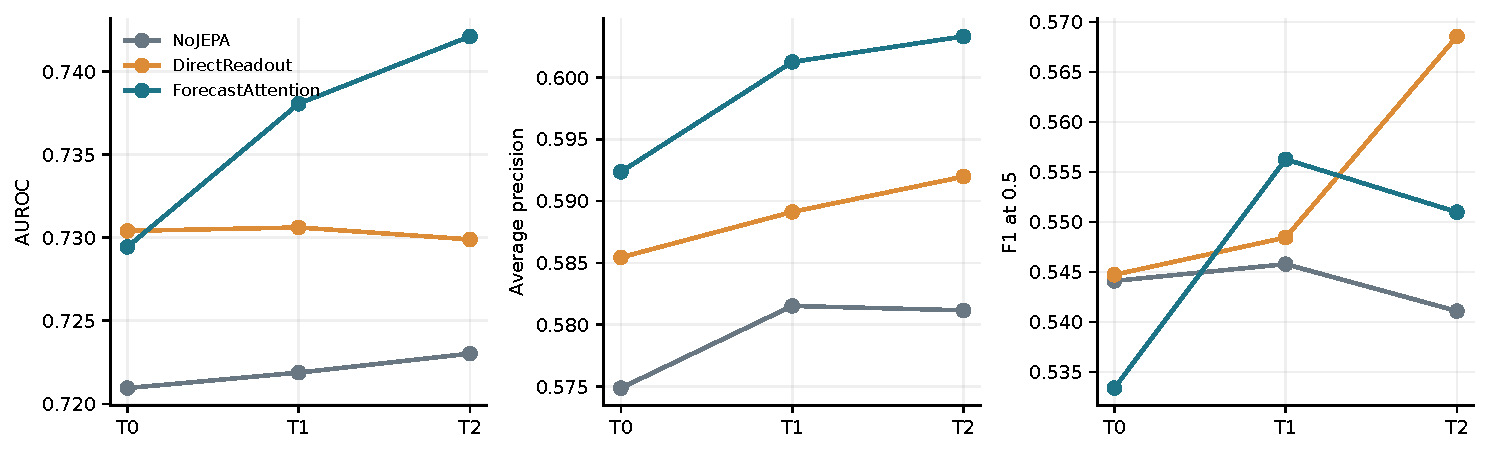
\includegraphics[width=\textwidth]{figures/landmark_performance.pdf}
\caption{Landmark-specific seed44 performance on the internal holdout. Each point averages metrics of five separately evaluated fold models. All landmarks use the same 175 patients. Lines connect landmark summaries and do not imply a statistically established temporal trend.}
\label{fig:landmarks}
\end{figure}

\subsection{Auxiliary supervision and forecast readout}
Adding future-state supervision while retaining direct readout increased mean AUROC by 0.0084, AP by 0.0097, and F1 by 0.0102 for \direct{} relative to \nojepa{}. Introducing the complete forecast-attention readout produced a further mean AUROC increase of 0.0062 and an AP increase of 0.0101 relative to \direct{}, accompanied by a mean F1 decrease of 0.0070. These two comparisons address different changes: the first isolates the auxiliary loss more closely, while the second changes both the classifier information pathway and its input representation.

The supplementary pooling comparison is provided in Table~\ref{tab:pooling}. Relative to \meanmodel{}, \fullmodel{} increased mean AUROC by 0.0017, AP by 0.0144, and F1 by 0.0011. At T0, however, its AUROC was lower by 0.0023 and its F1 was lower by 0.0113. The seed44 evidence therefore supports a modest descriptive aggregate difference between pooling choices, rather than a uniform attention advantage.

\subsection{Longitudinal change and calibration}
The observed T2--T0 AUROC difference was +0.0127 for \fullmodel{}, compared with +0.0021 for \nojepa{} and $-0.0005$ for \direct{}. The T1 value of \fullmodel{} lay between its T0 and T2 values. Because the same patients were evaluated at every landmark, these differences are not caused by changes in the evaluated patient set. They nevertheless reflect this trained configuration and do not establish that each individual's prediction improved or that added visits would be beneficial in another cohort.

Probability quality showed an unfavorable trade-off (Table~\ref{tab:calibration}). \fullmodel{} had higher mean NLL (0.6149), Brier score (0.2147), and ECE (0.1622) than \nojepa{} (0.5974, 0.2069, and 0.1310, respectively). Consequently, the AUROC and AP results should not be interpreted as improved calibrated risk estimation. No post-hoc calibration model was fitted in this analysis.
\begin{table}[t]
\centering
\caption{Calibration and probability accuracy, averaged over landmarks and five fold models for seed44. Lower is better. ECE uses ten equal-width bins.}
\label{tab:calibration}
\begin{tabular}{lrrr}
\toprule
Model & NLL & Brier & ECE \\
\midrule
NoJEPA & 0.5974 & 0.2069 & 0.1310 \\
DirectReadout & 0.5995 & 0.2073 & 0.1377 \\
ForecastAttention & 0.6149 & 0.2147 & 0.1622 \\
\bottomrule
\end{tabular}
\end{table}


\subsection{Conditional patient-level uncertainty}
The 95\% patient-bootstrap interval for mean AUROC was [0.6647, 0.8062] for \fullmodel{} and [0.6485, 0.7966] for \nojepa{}. The paired mean AUROC difference between these models was +0.0146, with interval [$-0.0062$, +0.0369]. The corresponding AP and F1 differences were +0.0198 [$-0.0161$, +0.0597] and +0.0032 [$-0.0339$, +0.0398]. Principal paired intervals included zero (Table~\ref{tab:bootstrap}), indicating that the observed differences remain uncertain even conditional on the fixed models. These intervals additionally omit the retrospective seed-selection uncertainty described in Section~\ref{sec:experiments}.

\section{Discussion}
\label{sec:discussion}
\subsection{What the matched comparisons establish}
The seed44 analysis shows a descriptive increase in mean AUROC and AP as the model progresses from direct prediction without future-state supervision to auxiliary-supervised direct prediction and then to forecast-attention readout. The first contrast is consistent with future-state supervision encouraging an observed-history representation that is useful for pCR prediction. The second is consistent with additional predictive value in a classifier that receives the forecast state and its change. However, the latter comparison also changes classifier width and pooling, so it cannot attribute the difference exclusively to a more accurate latent forecast. The supplementary mean-pooling control narrows the pooling question but exhibits only a small mean AUROC difference.

This distinction also changes how the model should be described. The main experiments do not reconstruct future MRI for classification and do not establish that an imagined image reproduces a patient's future anatomy. Rather, an auxiliary latent objective regularizes a representation, and the full classifier reads a predicted embedding. Moreover, the direct control named \nojepa{} retains the common fusion backbone and its transition queries. It is an ablation of future-state supervision, not proof that every world-model-related architectural component has been removed. Describing the actual information paths is more informative than relying on the experiment labels alone.

\subsection{Longitudinal prediction and the role of treatment context}
The full model's AUROC increased across T0--T2 in the selected seed, and the larger differences relative to the direct control occurred at later landmarks. One plausible explanation is that an observed response trajectory helps condition later-state forecasts. Another is that the additional forecast features or classifier capacity suit the later-prefix distribution. The current experiments do not distinguish these explanations. Forecast-quality analysis, frozen-forecast controls, parameter-matched direct classifiers, and prospective landmark-specific validation would help determine the mechanism.

Treatment is represented as an assigned-arm scenario assumed known at baseline. In the source protocol, T0 MRI preceded randomization; therefore, using the eventual assignment with T0 MRI is a retrospective conditional analysis and cannot be interpreted as a deployable prediction before allocation. The input does not encode the patient's verified delivered dose, dose reductions, actual cycle timing, adherence, or later treatment changes. Consequently, the framework should be interpreted as response prediction conditional on an encoded assignment, not as a simulator for treatment intervention. Comparing predictions under different assigned-arm tokens would not estimate causal treatment effects without additional assumptions, appropriate treatment data, and a separate causal analysis.

\subsection{Discrimination is not calibrated clinical utility}
The forecast-attention model's improved AUROC and AP coexisted with lower mean F1 than auxiliary-supervised direct readout and worse NLL, Brier score, and ECE than the control without future-state supervision. These discrepancies are expected to matter if probabilities are used to support decisions. AUROC measures ranking over thresholds, while F1 at 0.5 depends on a particular operating point; neither alone certifies useful clinical risk estimates. The model was selected by validation F1, not by a prespecified utility function. Independent assessment of calibration, clinically motivated operating points, and decision consequences is needed before suggesting a role in patient management. The attention maps also require separate validation before being interpreted as anatomical explanations.

\subsection{Limitations and requirements for a confirmatory study}
\label{sec:limitations}
The most immediate limitation is retrospective seed selection. Seed44 was chosen for manuscript presentation after multiple-seed results were available, including holdout results. A matched seed does not make this selection prospective. Patient bootstrapping quantifies variation in the evaluated patient sample conditional on the trained models, but cannot account for selection among seeds or the randomness of retraining. All reported model comparisons and intervals should therefore be considered exploratory. A confirmatory study should lock the model, seed policy, endpoints, and analysis before evaluating new patients.

The second limitation concerns the evaluation cohort and upstream independence. The holdout is an internal downstream split, not an external institution or independent prospective cohort. Twenty-nine of its patients had belonged to a development split in an earlier experimental lineage. Current supervised training uses the new patient-disjoint folds and does not warm-start from those earlier pCR models. Nevertheless, the patient-level overlap of the pretrained codec and localization-segmentation development data with the current holdout has not been fully established. This unresolved provenance prevents a claim that the complete pipeline has been assessed on entirely unseen patients at every stage.

Third, the fixed crop and preprocessing introduce constraints. A T0-derived localization window is used for all visits, and some predicted lesion components extend beyond the fixed field of view. Geometry and array-consistency checks do not substitute for anatomical review of segmentation or registration. The spatial window may underrepresent multifocal disease, chest-wall extent, or changes outside the crop. Complete T0--T2 availability is also required for holdout inclusion, whereas the development set retains incomplete histories. Performance may therefore differ for patients with missing interim MRI, and the missingness process may itself be associated with clinical factors.

Fourth, the present empirical comparison comprises matched internal variants. It does not yet establish performance against clinical-only models, conventional imaging biomarkers, independent longitudinal architectures, or contemporary published methods under the same split. Patient-subgroup analysis, scanner and site stratification, subtype-specific sensitivity, and the relationship between forecast error and classification error are also incomplete. The relatively small holdout, with 56 positive outcomes, limits the precision of those analyses and the principal paired estimates.

Finally, several reporting details still require confirmation from original clinical documentation: the exact pCR pathology definition and assessment workflow, actual patient-level acquisition intervals and treatment exposure, clinical-data adjudication, and the applicable ethics determination. The nominal stage timing is documented, but adherence and interval distributions have not yet been audited. These are explicit outstanding items in this draft rather than assumptions filled from common practice. Independent external validation, complete pretraining provenance, suitable external baselines, and a prespecified analysis would materially strengthen the evidence for a final Medical Image Analysis submission.

\section{Conclusion}
We investigated a latent forecasting framework for longitudinal pCR prediction from breast MRI using matched direct and forecast-based controls. In the retrospectively selected seed44 analysis, forecast-attention readout produced the highest mean AUROC and AP among the principal variants, while auxiliary-supervised direct readout retained the highest mean F1. The complete model's calibration was worse, and paired patient-bootstrap intervals included zero for the principal differences. The findings motivate further study of future-state supervision and forecast-based readout, with prospective model selection, stronger baselines, complete upstream provenance, and independent validation required before a confirmatory or clinical-use claim.

\section*{Data and code availability}
Source imaging collections are available through The Cancer Imaging Archive, subject to their applicable access conditions and licenses. The present derived manifests, processing lineage, and evaluation outputs are retained locally. \todo{Specify the public repository, versioned release, permitted derived-data artifacts, and access mechanism before submission; no public code-release claim is made in this draft.}
\section*{Ethics approval and consent}
\todo{Provide the original studies' ethics and consent statements and the local institutional determination for this secondary analysis, including an approval or exemption identifier where applicable. Public availability alone is not an ethics approval.}
\section*{Funding}
\todo{Provide grant numbers and the funders' roles, or confirm that no specific funding was received.}
\section*{Declaration of competing interest}
\todo{Obtain and insert the actual declarations from every author.}
\section*{CRediT authorship contribution statement}
\todo{Provide author names and agreed contributions; no authorship or contributions have been inferred.}
\section*{Declaration of generative AI and AI-assisted technologies in the manuscript preparation process}
During preparation of this initial draft, OpenAI Codex was used to organize source evidence, generate reproducible aggregate tables and figures, and assist with English drafting. \todo{All authors must review and edit the manuscript, verify every statement and reference, and finalize the disclosure under the journal's current policy before submission.}
\appendix
\section{Supplementary pooling and uncertainty analyses}
\label{sec:supplement}
The supplementary \meanmodel{} uses the same seed44, folds, observed-history protocol, future-state objective, and forecast classifier feature groups as \fullmodel{}, replacing spatial attention with mean pooling. It is reported separately from the three principal variants requested for the main analysis.
\begin{table}[t]
\centering
\caption{Supplementary pooling comparison using seed44. ForecastMean and ForecastAttention share forecast-based pCR readout and future-state supervision, and differ in spatial pooling.}
\label{tab:pooling}
\begin{tabular}{llrrr}
\toprule
Model & Landmark & AUROC & AP & F1 \\
\midrule
ForecastMean & T0 & 0.7317 & 0.5812 & 0.5446 \\
ForecastMean & T1 & 0.7367 & 0.5869 & 0.5523 \\
ForecastMean & T2 & 0.7361 & 0.5856 & 0.5405 \\
ForecastMean & Macro & 0.7348 & 0.5845 & 0.5458 \\
\midrule
ForecastAttention & T0 & 0.7294 & 0.5924 & 0.5334 \\
ForecastAttention & T1 & 0.7381 & 0.6012 & 0.5563 \\
ForecastAttention & T2 & 0.7421 & 0.6033 & 0.5510 \\
ForecastAttention & Macro & 0.7365 & 0.5990 & 0.5469 \\
\bottomrule
\end{tabular}
\end{table}

\begin{table}[t]
\centering
\caption{Exploratory paired patient-bootstrap intervals for three-landmark mean differences (2,000 shared patient resamples). Intervals condition on the fixed seed44 models; they exclude retraining and seed-selection uncertainty.}
\label{tab:bootstrap}
\small
\begin{tabular}{llr}
\toprule
Comparison & Metric & Difference [95\% interval] \\
\midrule
DirectReadout -- NoJEPA & AUROC & +0.0084 [-0.0051, +0.0219] \\
DirectReadout -- NoJEPA & AP & +0.0097 [-0.0128, +0.0315] \\
DirectReadout -- NoJEPA & F1 & +0.0102 [-0.0118, +0.0325] \\
ForecastAttention -- NoJEPA & AUROC & +0.0146 [-0.0062, +0.0369] \\
ForecastAttention -- NoJEPA & AP & +0.0198 [-0.0161, +0.0597] \\
ForecastAttention -- NoJEPA & F1 & +0.0032 [-0.0339, +0.0398] \\
ForecastAttention -- DirectReadout & AUROC & +0.0062 [-0.0129, +0.0268] \\
ForecastAttention -- DirectReadout & AP & +0.0101 [-0.0244, +0.0482] \\
ForecastAttention -- DirectReadout & F1 & -0.0070 [-0.0396, +0.0237] \\
\bottomrule
\end{tabular}
\end{table}

\begin{figure}[t]
\centering
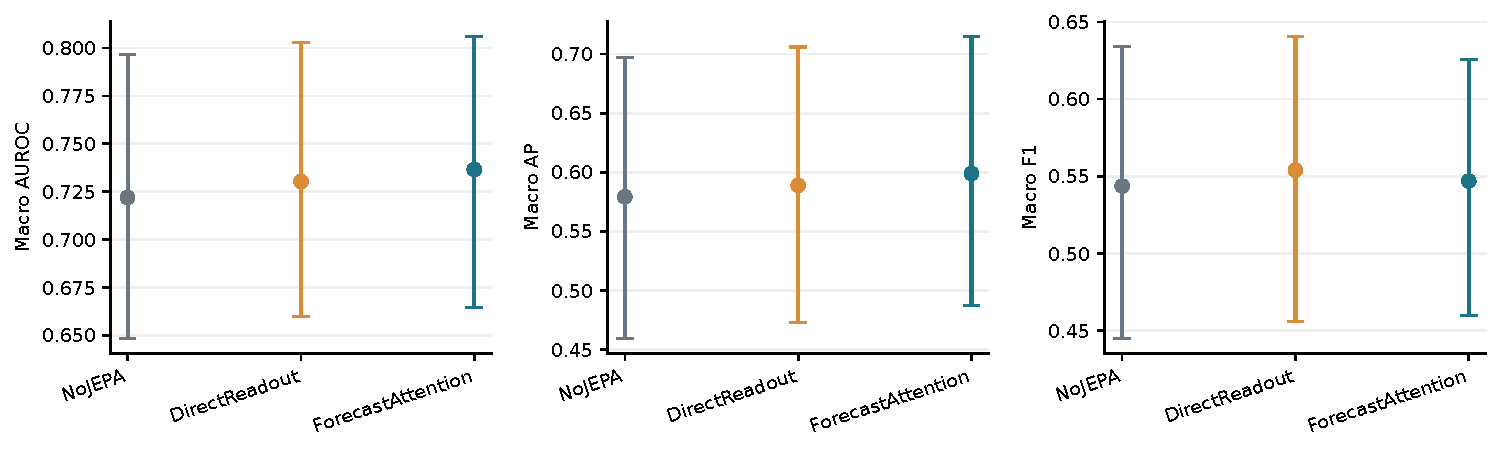
\includegraphics[width=\textwidth]{figures/patient_bootstrap.pdf}
\caption{Three-landmark mean metrics with exploratory 95\% percentile patient-bootstrap intervals. All 2,000 resamples preserve pairing across models, folds, and landmarks. Intervals describe patient-sampling uncertainty conditional on the trained seed44 models and do not account for seed selection or retraining.}
\label{fig:bootstrap}
\end{figure}
\section{Reproducibility and reporting items to complete}
The accompanying source package includes aggregate result CSV files, source-report hashes, the bootstrap procedure, figure-generation code, and a build script. It does not include patient identifiers, patient-level prediction rows, MRI volumes, or model checkpoints. All four model variants in this package use training seed44; the bootstrap random-number seed controls patient resampling only.

\todo{Before submission, complete the author and ethics statements; verify the pCR endpoint and visit timing; document codec and segmentation training-patient provenance; add matched external baselines and the locked multi-seed sensitivity analysis; audit external-cohort independence; and confirm the journal's current submission and anonymization requirements.}

\bibliographystyle{elsarticle-harv}
\bibliography{references}
\end{document}
